\subsection{UC22: Annullamento checkout}
\label{sec:UC22}
\begin{figure}[!ht]
    \caption{Diagramma di UC22: Annullamento checkout}
    \vspace{10px}
    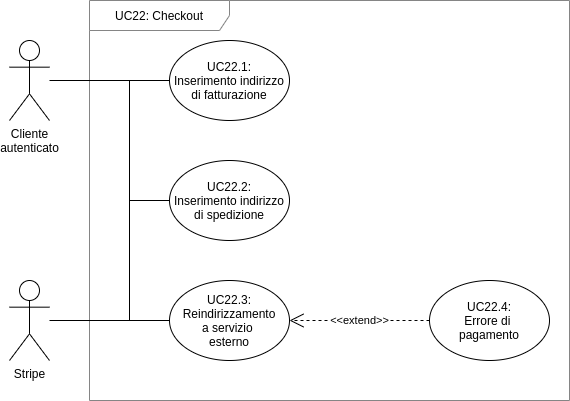
\includegraphics[scale=0.5]{../../../Images/AnalisiRequisiti/UC22}
    \centering
\end{figure}
\begin{itemize}
    \item \textbf{Descrizione:} visualizzazione di un errore per un fallimento nella fase di pagamento;
    \item \textbf{Attore Primario:} Stripe;
    \item \textbf{Precondizione:} il cliente ha inserito i dati del pagamento;
    \item \textbf{Input:} Stripe ritorna un errore nel risultato del pagamento;
    \item \textbf{Postcondizione:} viene visualizzato un messaggio di errore, successivamente il cliente viene reindirizzato alla sezione del checkout.
\end{itemize}
